% --------------------------------
%	LaTeX-File: MPP_Lab2.tex
% --------------------------------
%	Autor: 		Nils Parche
%	Dokument: 	MPP-1 LED-Pendel
%	Datum:		17.10.2016
% --------------------------------
%	Projekt-Name:	MPP-2 LED-Pendel
%
%
% --------------------------------


% include header

% --------------------------------
%	LaTeX-File: MPP_Lab2.tex
% --------------------------------
%	Autor: 		Nils Parche
%	Dokument: 	MPP-1 LED-Pendel
%	Datum:		17.10.2016
% --------------------------------
%	Projekt-Name:	MPP-2 LED-Pendel
%
%
% --------------------------------


%%%%%% header
\documentclass[a4paper,10pt]{scrartcl}		%layout (deutsch, A4, Schritgroesse)  ------>(scrartcl/scrreprt)

\usepackage[utf8]{inputenc}					% Erweiterte Schriftzeichen (ä, usw.)
\usepackage[ngerman]{babel}					% Deutsche Standart bei Dokumenterstellung (Inhaltsverzeichnis)
\usepackage[T1]{fontenc}					% Normale Schrift
\usepackage{amsmath}						% Mathefehle
\usepackage{graphicx}						% Einbinden von Grafiken

\usepackage{cite}							% Quellenangabe
\usepackage{float}							% Für das große H
\restylefloat{figure}						% in der figure

% Colors
\usepackage{color}
\definecolor{DarkPurple}{rgb}{0.4,0.1,0.4}
\definecolor{LightLime}{rgb}{0.3,0.5,0.4}
\definecolor{Blue}{rgb}{0.0,0.0,1.0}

% Quell-Code Darstellung
\usepackage{listings}
\usepackage{beramono}						% Text im Codebereich
\lstdefinestyle{styleNP}
{
language=C,
columns=flexible,
numbers=left,
frame=single,
frameround=tttt,
showstringspaces=false,						% 
basicstyle=\footnotesize\ttfamily,			% Schriftgröße verkleiner, weichere Darstellung
keywordstyle=\bfseries\color{DarkPurple},	% Farbe für while, for, etc.
commentstyle=\itshape\color{LightLime},		% Farbe für Kommentare
stringstyle=\color{Blue},					% Farbe für Strings
captionpos=b                    			% sets the caption-position to bottom
}

% Header and Footer Stuff
\usepackage{fancyhdr}
\pagestyle{fancy}
\fancyhead{}
\fancyfoot{}
\fancyfoot[R]{\thepage\ }

\usepackage{multicol}						% Einteilen einer Passage in mehrere Spalten
\usepackage[hidelinks]{hyperref}			% Rahmen bei Verknüpfungen unsichtbar
\usepackage{hyperref}						% Einfügen von Hyperlinks / Verknüpfungen

\usepackage[top=1.5in, bottom=1.75in, left=1.25in, right=1.25in]{geometry}
\usepackage{booktabs}

%%%%%% Dokument
\title{MPP-2 LED-Pendel}
\author{Nils Parche}
\date{\today}


%%%%%% Beginn des Dokuemteninhalts
\setlength{\parindent}{0pt}\begin{document}

%%%%%% Begin: Titlepage
% -- Titlepage
	\begin{titlepage}
		\begin{flushright}
			
\includegraphics[scale=0.08]{haw_logo_hd.png}\\
			{\tiny{Fakultät: Technik und Informatik || Department: Information und Elektrotechnik}}\\
			[2.5cm]
		\end{flushright}
		\begin{center}
			{\huge{\bfseries Laborbericht}}	\\
			[1.5cm]
% ---------------------------- Thema 
			{\Large{\bfseries  MPP-4 Serielle Schnittstelle}}\\		
			\line(1,0){400}	\\
			[0,1cm]
% --------------------------- Fach
			{\Large{\bfseries Labor Prozessortechnik}}	\\
			[1.5cm]
			\begin{table}[h]
				\begin{center}
					\begin{tabular}{r l}
% ----------------------------------------------------- Professor / Semstergruppe / Labordatum
						\small \textbf{Professor:}	&	\small \textbf{Prof. Dr.-Ing. K.-R. Riemschneider}\\[0.20cm]
						\small Semestergruppe:		&	\small E4			\\
						\small Datum des Labors:	&	\small 07.November 2016	\\
					\end{tabular}
				\end{center}
			\end{table}
			\vspace{0.5cm}
			\begin{table}[h]
				\begin{center}
					\begin{tabular}{r l}
% --------------------------------------------------------- Laborgruppenteilnehmer
						\small \textbf{Protokollant:}	&	\small 
						Nils Parche\\
						\small Matrikelnummer:			&	\small 2210363\\
						\small E-Mail:					&	\small 
						\href{mailto:nils.parche@haw-hamburg.de}{nils.parche@haw-hamburg.de}\\[0.30cm]
						\small \textbf{Assistent:}		&	\small 
						\textbf{Marvin Janz} \\
						\small Matrikelnummer:			&	\small 2245023\\
						\small E-Mail:					&	\small \href{mailto:marvin.janz@haw-hamburg.de}{marvin.janz@haw-hamburg.de}\\[0.30cm]

					\end{tabular}
				\end{center}
			\end{table}				
		\end{center}
	\end{titlepage}


\newpage
\listoftables
\listoffigures
\lstlistoflistings

\newpage

\tableofcontents
\newpage

	\section{Einleitung}
	
	Das letzte Labor in Mikroprozessortechnik beschäftigt sich mit der seriellen Übertragung. Es sollte eine Verbindung des Mikroprozessors mit dem PC über ein Hyper Terminal und einer RS 232 Schnittstelle erstellt werden. Mithilfe der erstellten Verbindung wurden anschließend drei verschiedene Übertragungsprozesse gemäß Aufgabenstellung realisiert.\\
	Diese waren:
	\begin{enumerate}
		\item Wiederholte Ausgabe eines Zeichens auf dem Hyper Terminal in Abhängigkeit:\label{Aufgabe 1} \begin{itemize}
			\item der Bitrate in $\frac{Bits}{sek}$
			\item der Anzahl der Datenbits
			\item der Paritätsgenerierung
			\item der Anzahl der Stoppbits
		\end{itemize}
	\item Ausgabe eines vorgegebenen Textes auf dem Hyper Terminal vom Mikrocontroller \label{Aufgabe 2}
	\item Übertragung eines frei wählbaren Textes vom Hyper Terminal zum \label{Aufgabe 3} Mikrocontroller unter der Beachtung, dass:\begin{itemize}
		\item Kein Zeichenüberlauf stattfindet 
		\item Schreibfehler korrigiert werden können
		\item Eine Echo Funktion aktiviert, oder deaktiviert werden kann
	\end{itemize}
	
	\end{enumerate}

\newpage

	\section{Aufgabenteil \ref{Aufgabe 1} Wiederholte Ausgabe eines Zeichens}\label{Aufgabenteil1}
	
	Für die wiederholte Ausgabe eines Zeichens wurden Übertragungen mit vier verschiedenen Einstellungen getätigt. Für jede Übertragung wurde jeweils das große \textbf{\textit{T}} verwendet.
	
	\begin{table}[h]
		\label{tab:EinstellungenZeichenübertragung}
		\centering
		\caption{Übersicht der Einstellungen zur Übertragung eines Zeichens an das Hyper Terminal}
		\begin{tabular}{|c|c|c|c|c|}
		Variante	&	Datenrate in Baud&	Datenbits&	Parität\footnotemark & Stopbits \\
				\toprule
				\bottomrule
		1	&		115200			&		 	8&	no parity	 		& 1\\
		2	&		115200 			& 			8&	even  				& 2\\
		3	&		19200			&			8&	odd					& 1\\
		4	&		2400			&			7&	no parity			& 1\\
				\hline
		\end{tabular}
	\end{table}
		\footnotetext{odd steht für ungerade Parität, even für gerade Parität}
	 
		Für die Umsetzung der Baud Rate in dem Mikrocontroller musste das UART Integer Baud Rate Divisor Register gesetzt werden. Die Einstellung der richtigen Baud Rate wurde mit der Formel
		
		\begin{equation}
			BRD = \frac{SysClk}{16 \cdot gewuenschte~Bitrate} 
		\end{equation}\cite{Skript_Riemschneider}
		berechnet.\\
		Das Ergebnis ist anschließend eine Bruchzahl. Diese wird in ihren ganzzahligen (integer) Teil und in ihren gebrochenen (fractional) Teil unterschieden.\\
		Der integer Teil wird in das 
		\begin{center}
			UARTx\_IBRD\_R \cite{Datenblatt_TM4C1294}
		\end{center}
		Register geschrieben.\\
	
		Der gebrochene Teil wird in das 
				\begin{center}
			UARTx\_FBRD\_R \cite{Datenblatt_TM4C1294}
		\end{center}
		Register geschrieben.

Für alle im Labor vorgenommenen Übertragungen wurde der UART6 verwendet. Des weiteren war der SysClk für die Berechnung der Baud Rate 25MHz. Dies musste so gewählt werden da für die Übertragung der Hauptoszillator des Prozessors initialisiert wurde.

\newpage

\subsection{Überlegung zur Ausgabe des übertragenen Signales}
Während des Laborversuches war es angedacht, wie auch im Kapitel \ref{GemessenesT} dargestellt, das übertragene Signal mit einem Oszilloskope zu analysieren. Eine im Vorfeld getätigte Überlegung wie der Signalverlauf von Beginn bis zum Ende der Übertragung aussehen würde. Diese wird im Folgenden in nummerisch aufsteigender Reihenfolge für das TTL Signal aufgelistet:
\begin{enumerate}
	\item Startbit: Der erste erscheinende Spannungssprung wird durch das Startbit entstehen. Dies kennzeichnet den Beginn der Übertragung.
	\item Datenbits: Direkt nach dem Startbit beginnt die eigentliche Übertragung des Signales. Hierbei muss auf die gewählte Länge des Datenbits geachtet werden. Handelt es sich um ein Zeichen aus dem ACSII-Code sind 7 Bits für den einfachen, sowie 8 Bits für den erweiterten Code (mit Umlauten/Sonderzeichen) von nöten. Andere Übertragungslängen erfordern eine sehr gute Abstimmung von Sender und Empfänger.\\
	\textbf{Wichtig bei der Übertragung der Datenbits: LSB first!}
	\item Paritätbit: Nach der Datenübertragung wird bei aktivierter Parität ein weiteres Bit übertragen. Je nach Einstellung auf odd oder even ist dies eins oder null.
	\item Stopbit: Als letztes wird ein Stopbit übertragen, welches die Beendigung der Datenübertragung kennzeichnet.
\end{enumerate}

Zu beachten ist auch, dass das RS232 Signal invertierend zur eigentlichen binären Logik ist. Dies bedeutet, dass eine logische 1 einen Spannungsabfall auf $\approx -10V$ hervorruft, während eine 0 einen Spannungsanstieg auf $\approx +10V$ verursacht.\\

\newpage

	\subsection{Programmalgorithmus für Variante 1} \label{ProgrammalotihmusAufgabenteil1}
	
	Da sich die vier Varianten für die Übertragung sich sehr stark ähneln, wurde davon abgesehen, diese jeweils aufzulisten.\\
	Im Folgenden wird die Variante 1 der Tabelle \ref{tab:EinstellungenZeichenübertragung} aus dem Kapitel \ref{Aufgabenteil1} komplett dargestellt:
	
	\lstinputlisting[style=styleNP, caption={Programmcode Übertragen eines Zeichens}, label={lst:vertikale_balken}]{../code/variante1.txt}
	
	\newpage
	
	\subsection{Parametereinstellung für Variante 2 , 3 , 4}
	
	Für die übrigen Varianten wurden folgende Parameter aus dem Ablauf in Kapitel \ref{ProgrammalotihmusAufgabenteil1} verändert.
	\begin{itemize}
	\item []	Zeile 32: Bitrate mit \# define BITRATE auf die gewählten Bits pro Sekunde gestellt
	\item []	Zeile 94: \begin{itemize}
		\item Veränderung der Bitlänge mit dem Befehl $UART\_LCRH\_WLEN\_x$
		\item Initialisierung der Paritätsgenerierung mit dem Befehl $UART\_LCRH\_PEN$
		\item Parität mit dem Befehl $UART\_LCRH\_EPS$ auf even gesetzt
		\item Parität durch das \textbf{Auslassen} des Befehles $UART\_LCRH\_EPS$ auf odd gesetzt
		\item Anzahl der Stopbits mit dem Befehl $UART\_LCRH\_STPx$ auf 1 oder 2 (anstelle von x) gesetzt
		\item Kein Stoppbit durch auslassen des Befehles $UART\_LCRH\_STP$
	\end{itemize}
	\end{itemize}
	
	\newpage
	
	\subsection{Auflistung der gemessenen Signale}\label{GemessenesT}
	
	Im Folgenden werden die im Labor festgehaltenen Messungen, welche über das Oszilloskop festgehalten wurden aufgelistet.
	
	\begin{figure}[h]
		\centering
		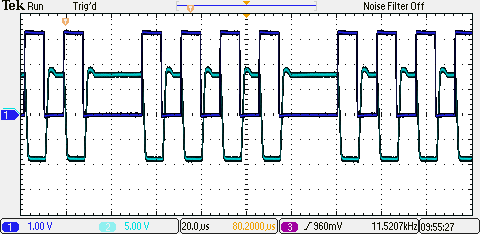
\includegraphics[width=1\linewidth]{../Bilder/Aufgabe1/Variante1}
		\caption{Serielle Übertragnung des Zeichens T mit der Einstellung der Variante 1}
		\label{fig:variante1}
	\end{figure}
	
	Abbildung \ref{fig:variante1}. Zu erkennen sind die beiden vom Typ TTL und RS 232. Das RS232 Signal verliert aufgrund der hohen Übertragungsrate an Qualität in der Anstiegszeit , sowie der Genauigkeit der Endwertspannung (es entsteht ein Überschwinger).
	
	\newpage
	
	\begin{figure}[h]
		\centering
		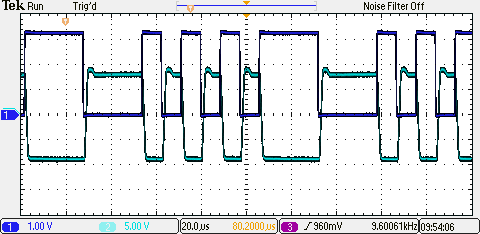
\includegraphics[width=1\linewidth]{../Bilder/Aufgabe1/Variante2}
		\caption{Serielle Übertragnung des Zeichens T mit der Einstellung der Variante 2}
		\label{fig:variante2}
	\end{figure}
	
	Abbildung \ref{fig:variante2}. Erneut ist , wie in Abbildung \ref{fig:variante1} aufgrund der hohen Baudrate Ein Qualitätsverlust im Bereich der slew rate , sowie ein Überschwinger zu erkennen.
	
	\newpage
	
	\begin{figure}[h]
		\centering
		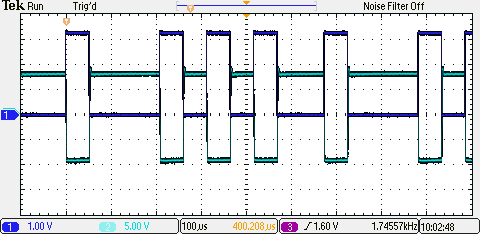
\includegraphics[width=1\linewidth]{../../Bilder/Variante3}
		\caption{Serielle Übertragung des Zeichens T mit der Einstellung der Variante 3}
		\label{fig:variante3}
	\end{figure}
	
	Abbildung \ref{fig:variante3}. Durch die verminderte Datenübertragungsrate ist die slew rate des RS 232 Signales verringert. Es ist allerdings weiterhin ein Überschwinger wie in Abb. \ref{fig:variante1}, sowie Abb. \ref{fig:variante2} zu beobachten. 
	
	\newpage
	
	\begin{figure}[h]
		\centering
		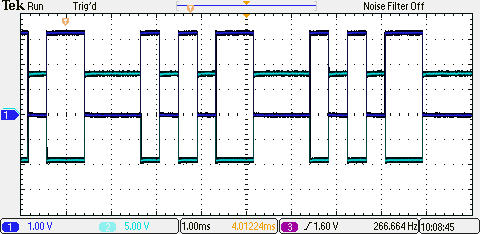
\includegraphics[width=1\linewidth]{../../Bilder/Variante4}
		\caption{Serielle Übertragnung des Zeichens T mit der Einstellung der Variante 4}
		\label{fig:variante4}
	\end{figure}

Abbildung \ref{fig:variante4}. Während des Versuches wurde bei dieser die geringste Baud-Rate eingestellt. Dies hat zur folge, dass die Qualität des RS 232 Signales von allen vier Varianten die beste darstellt. Es ist weder eine slew rate, noch ein Überschwinger des Signales zu beobachten.\\
\textbf{Zu beachten ist allerdings, dass bei einer verminderten Baud Rate die Anzahl der maximal zu übertragenen Zeichen ebenfalls verringert wird!}\\
Dieser Aspekt war für das vierte Labor nicht verlangt. 	
	\newpage
		\subsubsection{Handschriftliche Zeichnung der Signalverläufe}
	\begin{figure}[H]
\centering
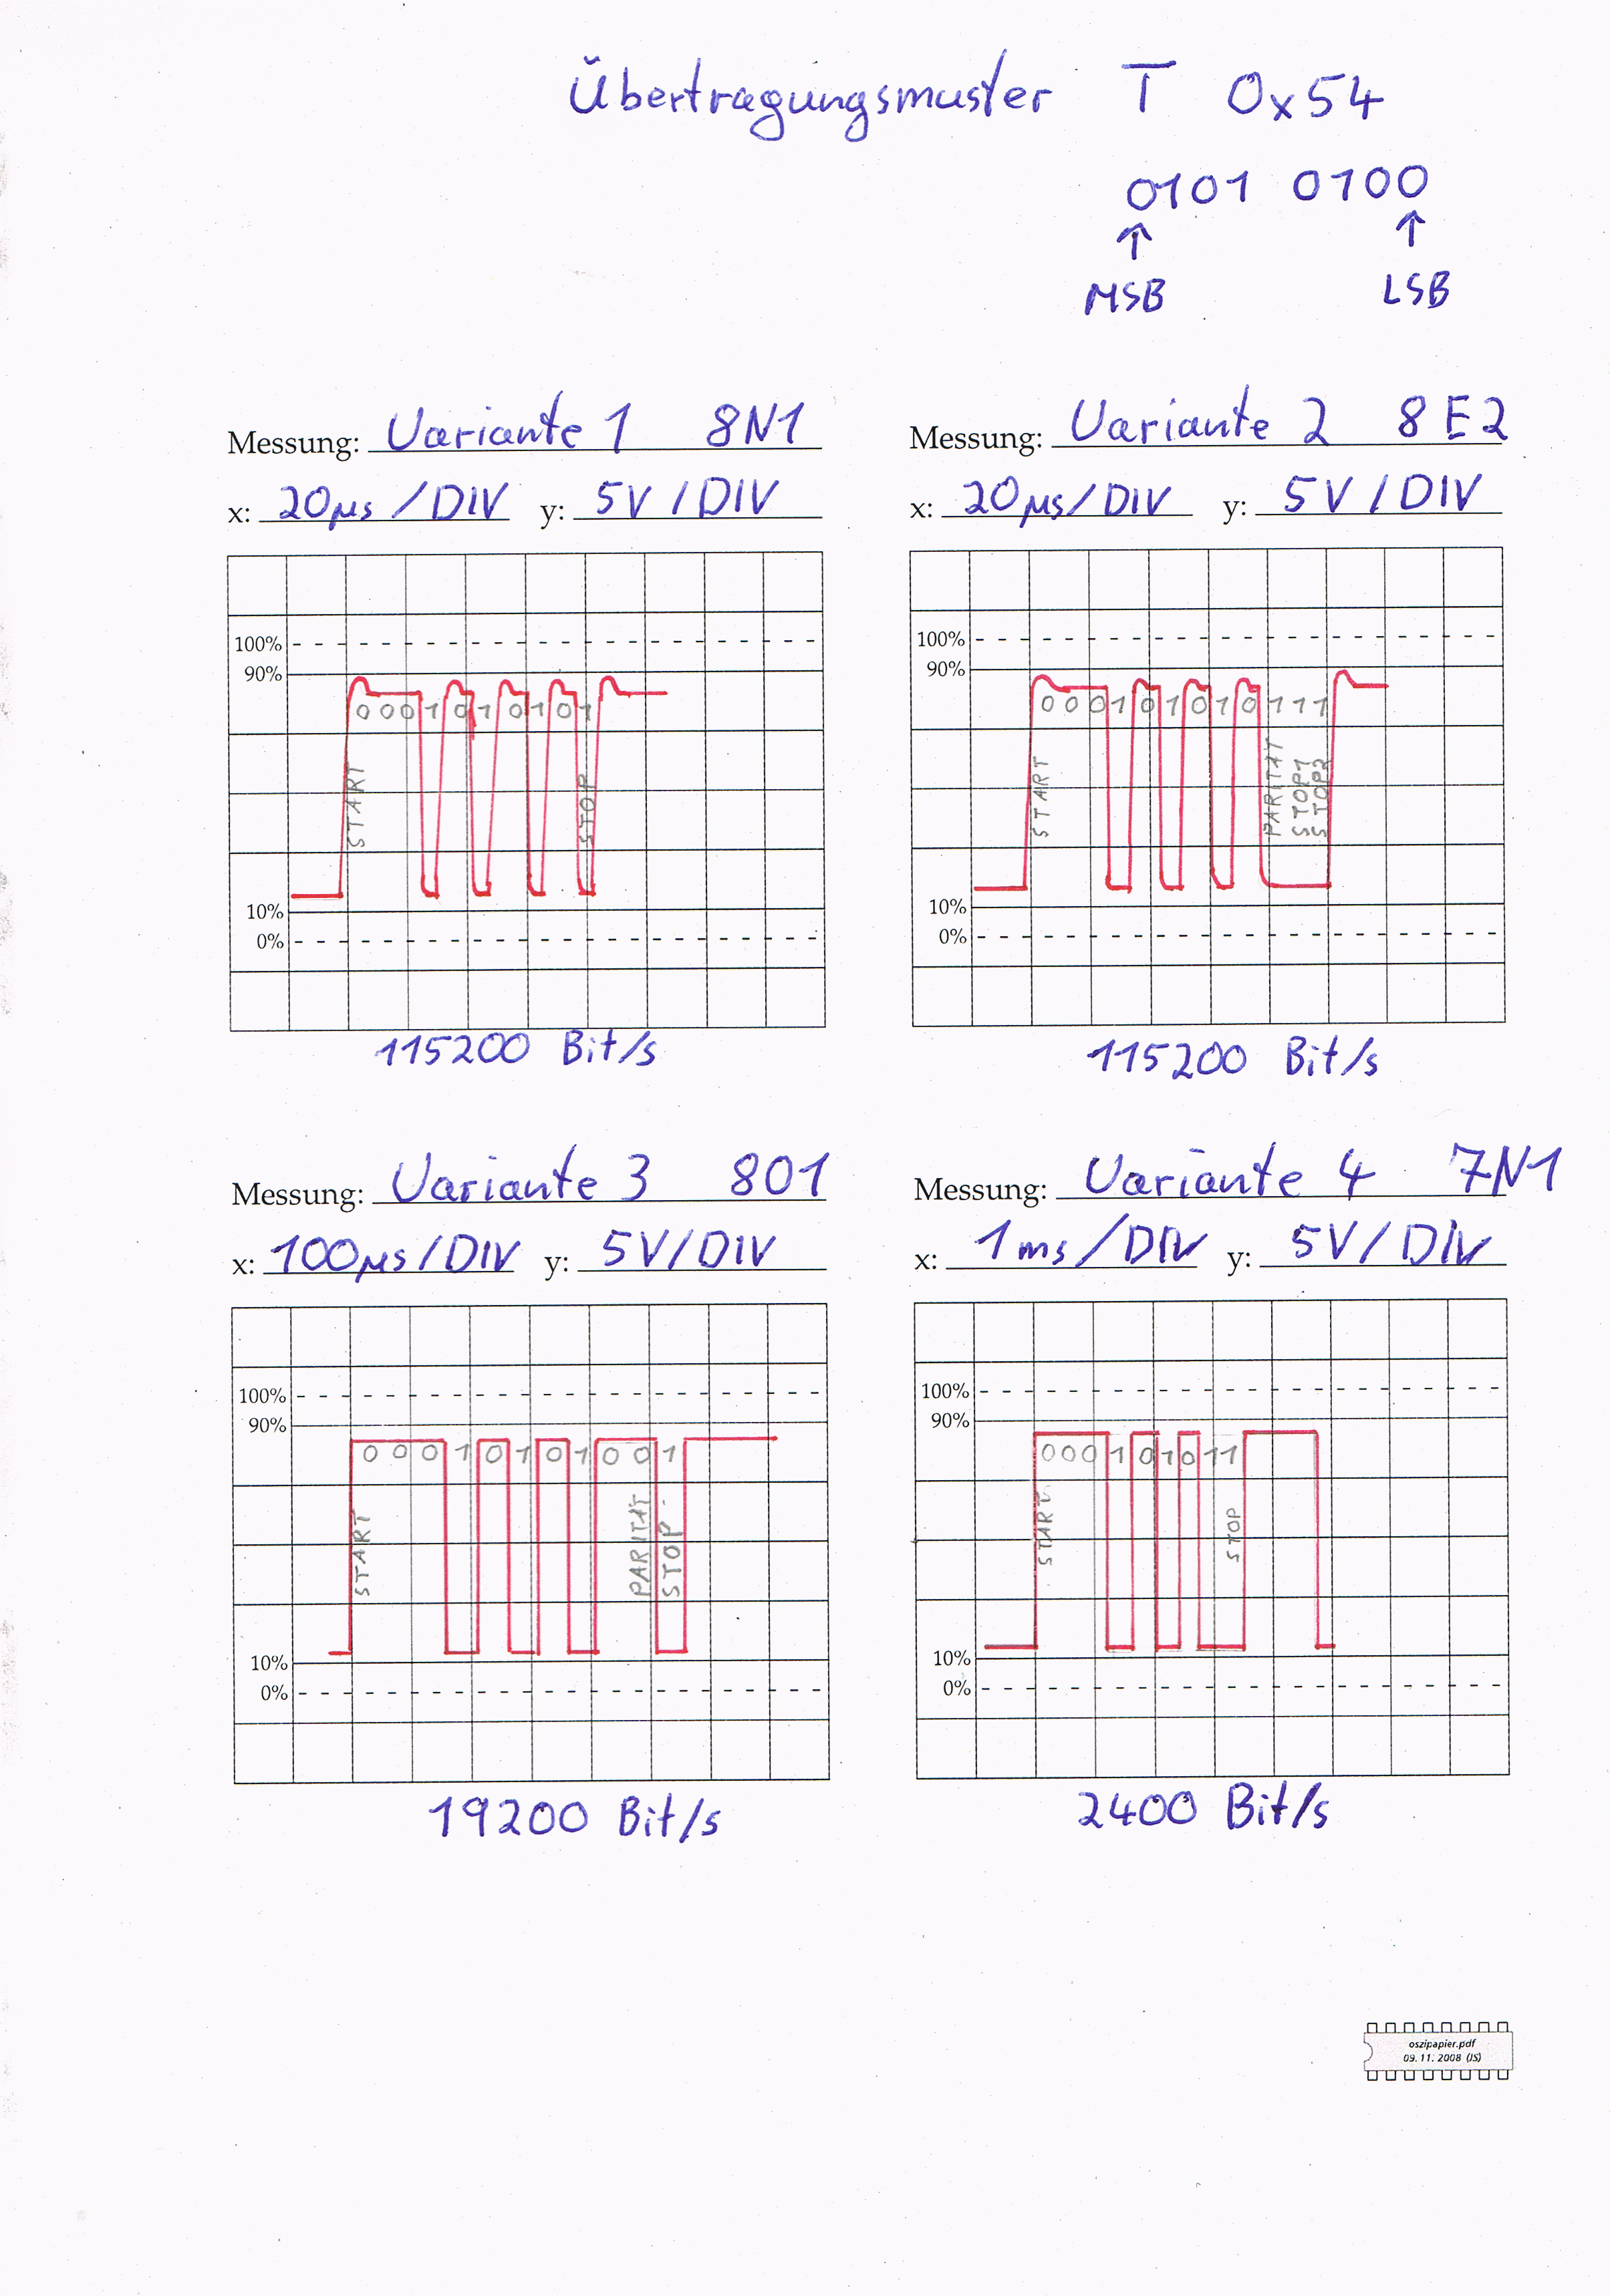
\includegraphics[width=0.8\linewidth]{../Bilder/Oszilloskop_Manuel}
\caption{Handschriftliche Zeichnung der Signalverläufe}
\label{fig:Oszilloskop_Manuel}
\end{figure}

	
	\newpage
	
	\subsection{Fazit}
	
	Bei der Übertragung ist es wichtig, einen klar und verständlichen Programmablauf zu programmieren, da die Grundeinstellung des Controllers immer die gleiche ist. Werden die fest einzustellenden Werte klar strukturiert, ist es anschließend nicht mehr kompliziert, unterschiedliche Übertragungsparameter einzustellen. Während der Messungen war zu erkennen, dass das eigentliche Serielle Ausgangssignal in seiner Qualität immer gleich blieb, während sich die Umsetzung auf ein RS 232 Signal mit der Baud Rate veränderte. War diese hoch, litt die Umsetzung an Überschwingern und es konnte eine Anstiegs-, sowie Abfallzeit der Flanken beobachtet werden.

	\section{Aufgabenteil \ref{Aufgabe 2} Ausgabe einer Zeichenfolge}
	\subsection{Beschreibung und Lösungsansatz}  

Der Aufgabenteil 2 verlangte es, einen vorgegebenen Text auf der Konsole des Hyper Terminals auszugeben. Der zu übertragenen Text lautete:

\begin{flushleft}
\textbf{\textit{Praktikum Serielle Uebertragung vom 19.12.2016.}\\
	\bigskip
	\textit{Versuchsteilnehmer:}\\
	\bigskip
	\textit{Nils Parche}\\
	\textit{Marvin Janz}}\\
\end{flushleft}

Die Konfiguration des Controllers wurde dabei aus der ersten Aufgabe übernommen. Die vorgenommen Einstellungen waren: 
\begin{itemize}
	\item Für die Baudrate: $9600 \frac{Bit}{s}$
	\item Für den System Clock 25 MHz (Hauptoszillator)
	\item UART6 für die serielle Übertragung gewählt
	\item Konfiguration des $UART6\_LCRH\_R$ Registers:\cite{Datenblatt_TM4C1294} \begin{itemize}
		\item $UART\_LCRH\_WLEN\_7$ Übertragen von 7 Datenbits
		\item $UART\_LCRH\_PEN$ Initialisieren der Paritäts Abfrage
		\item $UART\_LCRH\_EPS$ Einstellen gerader Parität
		\item Kein Stoppbit durch auslassen des Befehles $UART\_LCRH\_STP$
	\end{itemize}
\end{itemize}

Der zu übertragenen Text wurde, mit Formatierung, in ein char Array geschrieben und über eine for Schleife an das Hyper Terminal  übergeben. Siehe dazu Programmcode Listing \ref{lst:gewaehlterText}, Zeile 92-99.

\newpage

	\subsection{Programmalgorithmus}
	Folgender Programmalgorithmus kam zum Einsatz:
	
		\lstinputlisting[style=styleNP, caption={Programmcode Übertragen eines ausgewählten Textes}, label={lst:gewaehlterText}]{../code/datenausgabe.txt}

	\subsection{Struktogramm Aufgabe \ref{Aufgabe 2}}

	\begin{figure}[H]
		\centering
		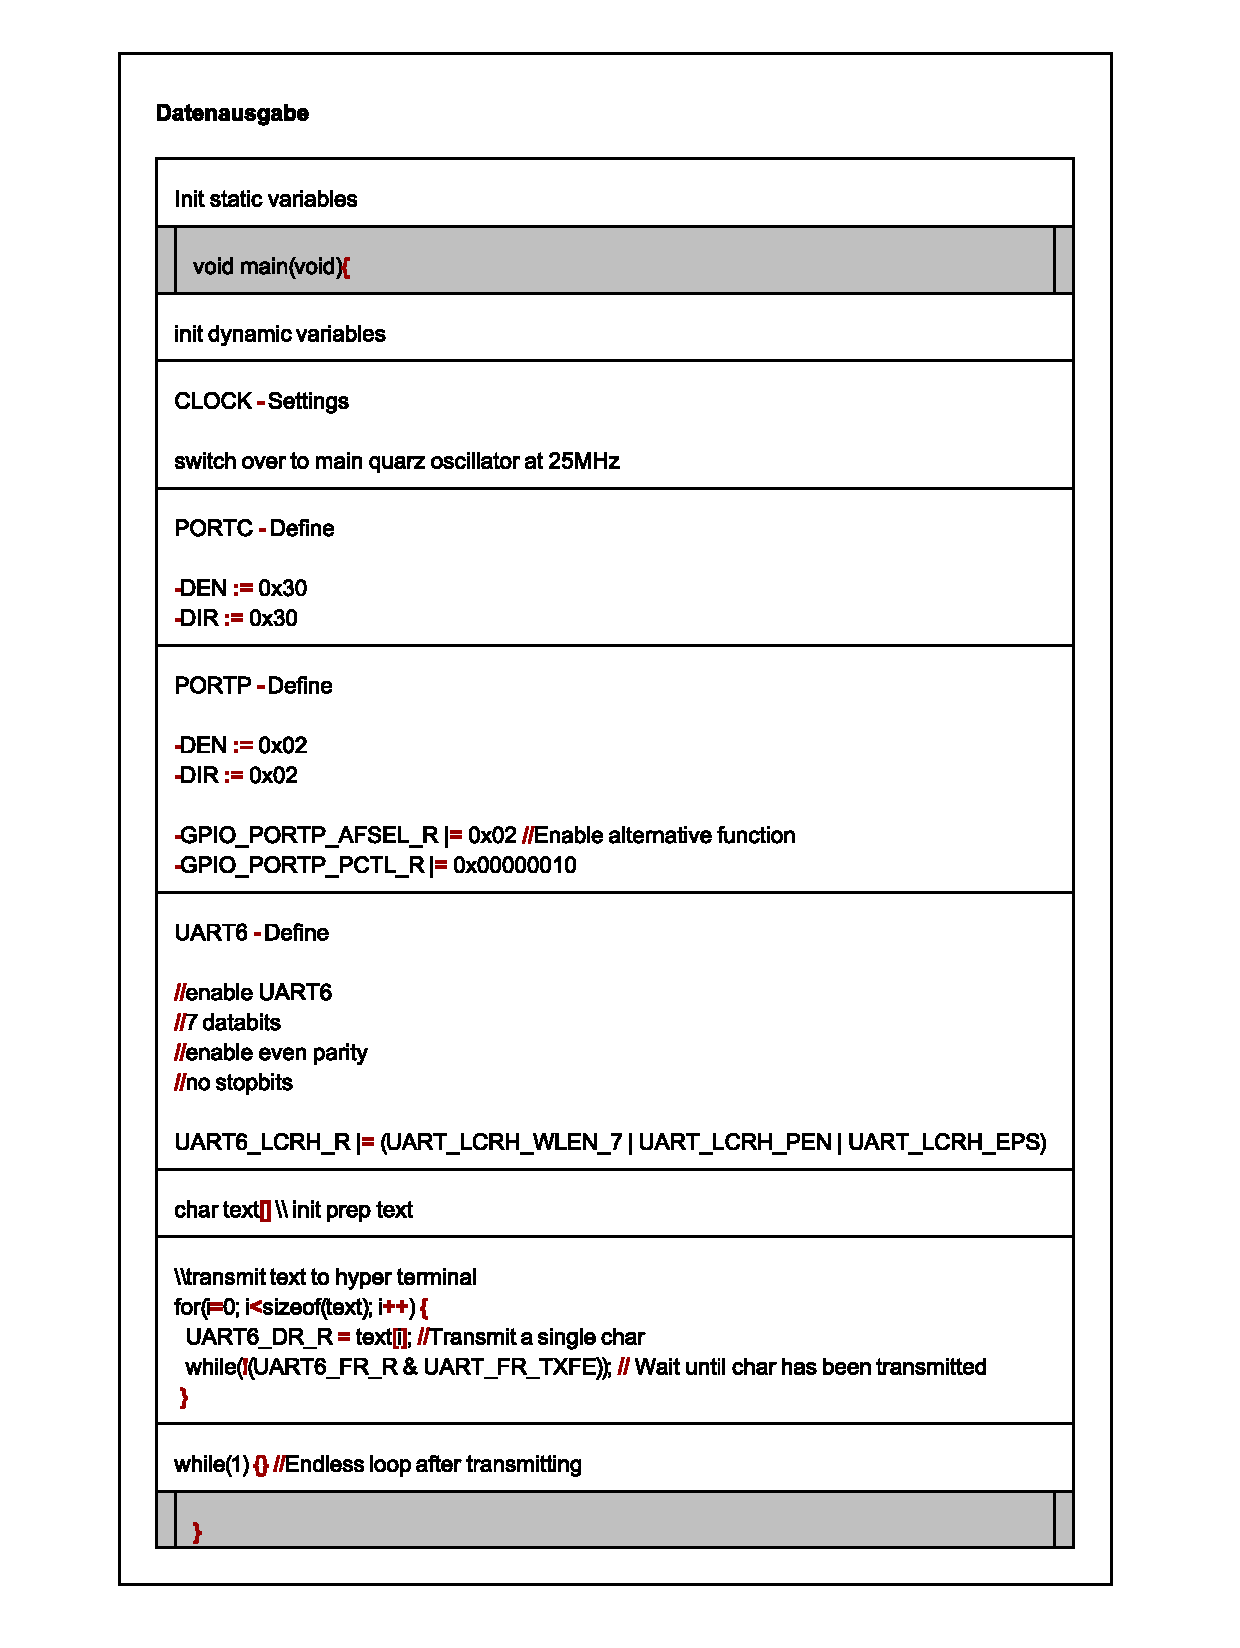
\includegraphics[width=0.9\linewidth]{../nassischneider/Datenausgabe_pdf}
		\caption{Nassi Schneidermann Diagramm zur Datenausgabe}
		\label{fig:datenausgabepdf}
	\end{figure}

\newpage
	\subsection{Fazit}
	
	Die Übertragung eines vorgewählten Textes erwieß sich als nicht kompliziert. Durch die vorhergehenden Aufgaben konnte die Einstellung des Controllers erneut ohne große Komplikationen vorgenommen werden.  Die Übertragung der Zeichenkette erforderte hingegen etwas Überlegung. Es ist mit der hier aufgeführten Lösung zum Beispiel schwierig eine dynamische Eingabe durch einen Benutzer zu übersetzten. Das Hauptproblem stellt hierbei die Formatierung durch z.B. Zeilenumbrüche dar.
	
	\newpage
	
	\section{Aufgabenteil \ref{Aufgabe 3} Empfangsprogramm}
	
	\subsection{Beschreibung und Lösungsansatz}
	Es soll ein Programm entwickelt werden mit dem es möglich ist Zeichen über die Serielle Schnittstelle des Controllers einzulesen. Die Parameter der Seriellen-Schnittstellen entsprechen dem des vorherigen Aufgabenteils (9600 bit/s, 7E1). Um den Speicherbedarf, der mit der Anzahl zu speichernden Zeichen begrenzt wird, wurde ein Array der Größe 16 als Einlesespeicher festgelegt. Des weiteren sollen die nachfolgenden Punkte in den Programmablauf eingebunden werden.
	
	\begin{itemize}
		\item \textbf{Es sollen Schreibfehler mit dem Zeichen Backspace (0x08) korrigiert werden können:}\\
		Jedes eingelesene Zeichen wird als ASCII-Code repräsentiert. Die Backspace-Taste besitzt den Code 0x08 und somit kann dieser abgefragt werden. Im Programmablauf wird bei erkennen der Backspace-Taste das vorherige Zeichen gelöscht. Zusätzlich wird die Position des Cursor um eine Stelle nach vorne versetzt, es sei denn der Cursor befindet sich bereit am Anfang.
		\item \textbf{Die Eingabe kann beendet werden mit \glqq End of file\grqq~Tastatureingabe (Ctrl + d):}\\
		Durch die Beendigung der Eingabe (Tastatur Ctrl+d) wird im Programmablauf das einlesen abgebrochen und der aktuelle Lesespeicher zur Kontrolle an den Terminal zurückgesendet.
		\item \textbf{Mit einem externen Schalter kann zwischen non-Echo- und Echo-Modus gewählt werden:}\\
		Bei aktivem Echo-Modus wird jedes Empfangendes Zeichen sofort an den Terminal zurück gesendet. Es dient der Visualisierung der Übermittelten Zeichen.
		
	\end{itemize}
	
	\subsection{Programmalgorithmus}
	Das Programm wurde so angelegt, dass nur maximal 15 Zeichen in einem Speicher geladen werden können. Durch diese Randbedingung ist eine bedingte Schleife erforderlich, die genau 15 Werte einließt oder mit der Tastatureingabe \glqq End of file\grqq~ beendet wird. Sollte nach dem 15 Wert weitere Zeichen übermittelt werden, wird eine Fehlermeldung mit den aktuellen Lesespeicher an den Terminal übermittelt. Erst nachfolgend wird das neu empfangende Zeichen in den Speicher geladen.\\
	Mit der Backspace-Taste kann die Eingabe der zuvor getätigten Zeichen gelöscht werden. Im Programmablauf wird bei jeder erkannten BS-Taste der Inhalt des Empfangsspeichers an der vorherigen [i-1] Position gelöscht, es sei den die aktuelle Position ist i == 0. Die letzte Spalte des Array wird benötigt um den String abzuschließen (0x00). Ohne diese Operation könnten auf dem Speicherinhalt keine komfortablen String-Funktionen angewandt werden.


	\newpage
	
	\subsection{Struktogram und Programmcode}
	
		\begin{figure}[H]
		\centering
		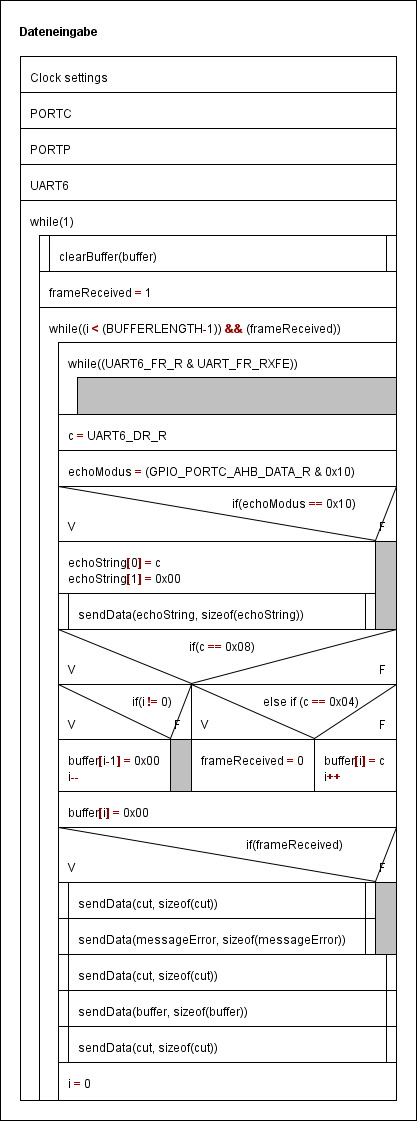
\includegraphics[width=0.5\linewidth]{../Bilder/Struktogramm_Dateneingabe}
		\caption{Nassi-Schneiderman Struktogram - Empfangsprogramm}
		\label{fig:Struktogramm_Dateneingabe}
		\end{figure}

	\newpage

		\lstinputlisting[style=styleNP, caption={Programmcode Empfangsprogramm}, label={lst:Empfangsprogramm}]{../code/dateneingabe.txt}
	
	\subsection{Fazit}
	Bei der verwendeten Bit-Rate ist eine Verzögerungszeit zwischen der Eingabe und der Ausgabe von mehreren ASCII-Zeichen bemerkbar, sodass sich diese Konfiguration nicht für eine schnelle Datenübermittlungen eignet.
	
	
	\bibliography{bibfile}{}
	\bibliographystyle{plain}
	
\end{document}
